\documentclass[aspectratio=169,11pt]{beamer}
% ==========================================================================
%  KSA lecture-slide theme  =  stock beamer "Boadilla"  +  KSA colour theme
%  brand colours sampled from the official KSA symbol mark:
%    Deep Prussian Blue  #2E3192   (지성 - intellect)
%    Golden Gray         #D6CBB1   (감성 - sensibility)
%  Engine: XeLaTeX.  Usage:
%    \documentclass[aspectratio=169,11pt]{beamer}
%    \input{../../theme/ksa-theme.tex}
%  Each deck lives in its own slides/kor/<deck>/ folder together with its
%  own images; ../../figs/ is kept only as a fallback for the shared cache.
% ==========================================================================

\usepackage{fontspec}
\usepackage{amsmath,amssymb}
\usepackage{graphicx}
\graphicspath{{figs/}{./}{../../../figs/}}
\usepackage{booktabs}
\usepackage{listings}
\usepackage{varwidth}

% ---- fonts (no ctex/xeCJK on this box -> fontspec drives CJK directly) -----
\defaultfontfeatures{Ligatures=TeX}
\setmainfont{Noto Sans CJK KR}
\setsansfont{Noto Sans CJK KR}
\setmonofont{Noto Sans Mono CJK KR}[Scale=0.92]

% ---- base theme: stock Boadilla ------------------------------------------
\usetheme{Boadilla}
\usefonttheme{professionalfonts}
\setbeamertemplate{navigation symbols}{}

% ---- KSA colour theme (recolour the stock theme) --------------------------
\definecolor{ksablue}{HTML}{2E3192}
\definecolor{ksabluedk}{HTML}{20226A}
\definecolor{ksagold}{HTML}{D6CBB1}
\definecolor{ksagolddk}{HTML}{A9976B}
\definecolor{ksared}{HTML}{C0392B}
\definecolor{ksagray}{HTML}{5B5B5B}

\setbeamercolor{structure}{fg=ksablue}
\setbeamercolor{alerted text}{fg=ksared}

\setbeamercolor{palette primary}{fg=white,           bg=ksablue}
\setbeamercolor{palette secondary}{fg=white,         bg=ksablue!85!black}
\setbeamercolor{palette tertiary}{fg=white,          bg=ksabluedk}
\setbeamercolor{titlelike}{fg=ksablue}
\setbeamercolor{frametitle}{fg=ksablue,bg=}
\setbeamercolor{title}{fg=ksablue}
\setbeamercolor{author}{fg=ksagray}
\setbeamercolor{institute}{fg=ksagray}
\setbeamercolor{block title}{fg=white,bg=ksablue}
\setbeamercolor{block body}{fg=black!85,bg=ksablue!6}
\setbeamercolor{item}{fg=ksablue}
\setbeamercolor{section in toc}{fg=black!85}

\setbeamerfont{frametitle}{series=\bfseries}
\setbeamerfont{title}{series=\bfseries}

% ---- footline:  KSA mark | "Made by ..." | n / N   (matches reference) ----
\newcommand{\ksacredit}{}
\setbeamertemplate{footline}{%
  \hbox{%
    \begin{beamercolorbox}[wd=.18\paperwidth,ht=2.6ex,dp=1.5ex,leftskip=1.1em]{}%
      \raisebox{-0.35ex}{\includegraphics[height=2.0ex]{ksa-logo.png}}%
    \end{beamercolorbox}%
    \begin{beamercolorbox}[wd=.64\paperwidth,ht=2.6ex,dp=1.5ex,center]{}%
      {\scriptsize\color{ksagray}\ksacredit}%
    \end{beamercolorbox}%
    \begin{beamercolorbox}[wd=.18\paperwidth,ht=2.6ex,dp=1.5ex,rightskip=1.1em]{}%
      \hfill{\scriptsize\color{ksablue}\insertframenumber\,/\,\inserttotalframenumber}%
    \end{beamercolorbox}%
  }%
  \vskip2pt
}

% ---- section divider: stock \sectionpage, KSA-coloured -------------------
\setbeamertemplate{section page}{%
  \begingroup\centering
    {\color{ksagolddk}\rule{0.16\paperwidth}{1pt}}\par\vskip1.0em
    {\usebeamerfont{title}\color{ksablue}\insertsectionhead\par}\vskip1.0em
    {\color{ksagolddk}\rule{0.16\paperwidth}{1pt}}\par
  \endgroup
}
\AtBeginSection[]{\begin{frame}[plain,noframenumbering]\vfill\sectionpage\vfill\end{frame}}

% ---- code listings ------------------------------------------------------------
\lstdefinestyle{ksa}{%
  basicstyle=\ttfamily\scriptsize,
  keywordstyle=\color{ksablue}\bfseries,
  commentstyle=\color{ksagray}\itshape,
  stringstyle=\color{ksagolddk},
  numberstyle=\tiny\color{ksagray},
  backgroundcolor=\color{ksablue!6},
  frame=leftline, framerule=1.4pt, rulecolor=\color{ksablue},
  xleftmargin=1em, aboveskip=0.8em, belowskip=0.4em,
  showstringspaces=false, breaklines=true, language=Python,
}
\lstset{style=ksa}

% ---- handy macros -----------------------------------------------------------
\newcommand{\kb}[1]{\textbf{\color{ksablue}#1}}   % blue keyword
\newcommand{\kq}[1]{\textbf{\color{ksared}#1}}    % red key-question

\setbeamerfont{title}{series=\bfseries,size=\fontsize{24}{30}\selectfont}
\setbeamerfont{subtitle}{series=\bfseries,size=\fontsize{14}{18}\selectfont}
\setbeamerfont{author}{size=\normalsize}
\setbeamerfont{institute}{size=\small}
\graphicspath{{figs/}{../../../../assets/}}
\makeatletter
\newcommand{\markpage}[1]{\protected@write\@auxout{}{\string\newlabel{#1}{{\the\c@framenumber}{}}}\hypertarget{#1}{}}
\newcommand{\pref}[1]{\hyperlink{#1}{\textcolor{ksagolddk}{(p.\ref{#1})}}}
\makeatother

\renewcommand{\ksacredit}{Machine Learning 1 \,\textperiodcentered\, 정규화 L1 · L2}
\title{정규화: L1 · L2 (Ridge · Lasso)}
\subtitle{큰 가중치에 벌금을 매겨 과대적합을 막는다}
\author{Machine Learning 1}
\institute{한국과학영재학교 (KSA)}
\date{}
\begin{document}
\begin{frame}[plain,noframenumbering]\titlepage\end{frame}

% --- 오늘의 질문
\begin{frame}{오늘의 질문}
\vfill
\centering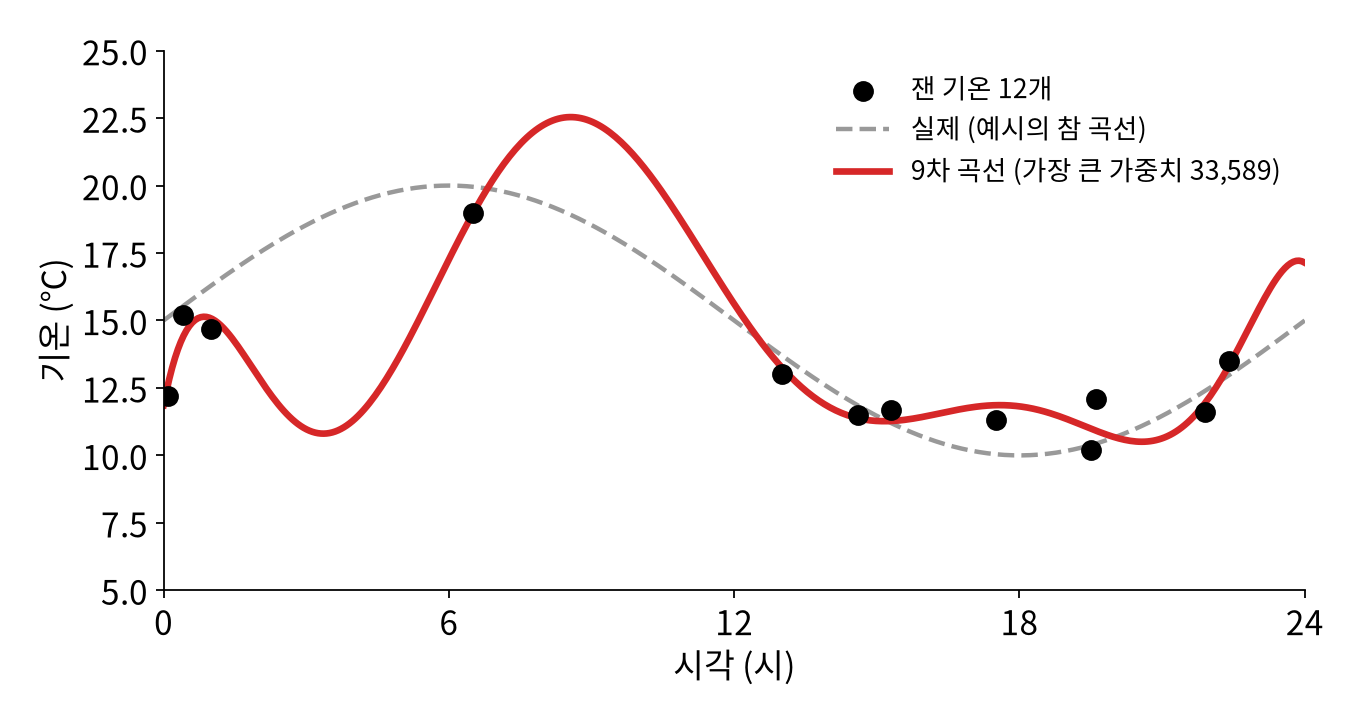
\includegraphics[width=0.62\linewidth]{rg_hook.png}\par\vskip0.2em
{\large 하루 기온 12번에 9차 곡선. \kq{가장 큰 가중치가 33,589.} 이 곡선을 믿을 수 있을까?}
\vfill
\note{하루 동안 기온을 12번 재서 점으로 찍었습니다. 회색 점선이 실제 기온 변화입니다. 예시 데이터라서 정답을 알고 있습니다. 여기에 9차 다항식을 맞췄더니 빨간 곡선이 나왔습니다. 잰 점은 거의 다 지나가는데, 점이 없는 오전 시간대에서 크게 출렁입니다. 가중치를 보면 가장 큰 것이 3만 3천이 넘습니다. 1주차에 본 과대적합입니다. 오늘은 차수를 낮추지 않고도 이런 곡선을 길들이는 방법, 정규화를 배웁니다.}
\end{frame}

% --- 과대적합 복습
\begin{frame}{점은 맞히는데, 실제와는 3.2 도 어긋난다}
\vfill
\centering
{\Large\begin{tabular}{lcc}
 & 잰 기온 12개와 오차 & 실제 기온과 오차\\\hline\\[-0.8em]
9차 곡선 & \kb{0.57 도} & \kq{3.2 도}
\end{tabular}}\vskip1.0em
{\large 측정 데이터 오차는 작은데 새 시각 오차는 크다 \quad = \quad \textbf{과대적합}}\\[0.6em]
{\large 증상: 가중치가 \kq{엄청나게 크다} (큰 양수와 큰 음수가 상쇄하며 점을 억지로 지난다)}
\vfill
\note{숫자로 보면 분명합니다. 잰 기온 12개와의 오차는 평균 0.57도로 작습니다. 그런데 하루 전체에서 실제 기온과 비교하면 3.2도나 어긋납니다. 측정 데이터에서는 잘 맞고 새 데이터에서는 틀리는 과대적합입니다. 과대적합된 다항식에는 늘 같은 증상이 있습니다. 가중치가 엄청나게 커서, 큰 양수 항과 큰 음수 항이 서로 상쇄하면서 점을 억지로 지나갑니다. 점 사이에서는 상쇄가 깨져 크게 출렁입니다.}
\end{frame}

% --- 정규화 식
\begin{frame}{정규화: 손실에 가중치 벌금을 더한다}
\markpage{loss}
\vfill
\centering
{\LARGE\[ J(\mathbf{w}) = \underbrace{\frac{1}{m}\sum_{i=1}^{m}\big(h(x^{(i)}) - y^{(i)}\big)^2}_{\text{error}} + \underbrace{\textcolor{ksared}{\lambda}\,R(\mathbf{w})}_{\text{penalty}} \]}\vskip0.4em
\renewcommand{\arraystretch}{1.3}
{\large\begin{tabular}{lll}
\kb{L2 (릿지, Ridge)} & $R = \sum_j w_j^2$ & 큰 가중치일수록 벌금이 제곱으로\\
\kb{L1 (라쏘, Lasso)} & $R = \sum_j |w_j|$ & 가중치 크기에 비례\\
\textcolor{ksared}{$\lambda$} & 벌금의 세기 & 0 이면 정규화 없음, 클수록 가중치가 작아진다
\end{tabular}}\vskip0.3em
{\small 절편 $w_0$ 에는 벌금을 매기지 않는다 (전체를 위아래로 옮기는 것은 과대적합과 상관없으니까)}
\vfill
\note{정규화는 손실 함수에 가중치 벌금을 하나 더하는 것입니다. 원래의 오차 제곱 평균에 람다 곱하기 벌금을 더합니다. 이제 경사하강법은 오차를 줄이면서 동시에 가중치를 작게 유지해야 합니다. 가중치를 크게 쓰면 손해니까요. 벌금의 종류가 둘 있습니다. 가중치 제곱의 합을 쓰면 L2, 릿지라고 하고, 절댓값의 합을 쓰면 L1, 라쏘라고 합니다. 람다는 벌금의 세기입니다. 0이면 정규화가 없고, 클수록 가중치가 작아집니다. 절편은 곡선 전체를 위아래로 옮길 뿐이라 벌금에서 뺍니다.}
\end{frame}

% --- 손으로
\begin{frame}{손으로 한 번: 릿지의 정답 식}
\markpage{hand}
\vfill
\centering
{\Large\[ \mathbf{w} = \big(X^\top X + \lambda D\big)^{-1} X^\top \mathbf{y} \qquad D = \text{diag}(0, 1, \dots, 1) \]}\vskip0.4em
{\large 점 3개 $x = 1, 2, 3$, \; $y = 3, 5, 7$ \; (정확히 $y = 1 + 2x$)}\vskip0.4em
\renewcommand{\arraystretch}{1.3}
{\Large\begin{tabular}{ccc}
$\lambda$ & $(w_0,\ w_1)$ & \\\hline
0 & $(1,\ 2)$ & 정규방정식 그대로\\
2 & $(3,\ 1)$ & 기울기가 절반으로\\
10 & $(4.33,\ 0.33)$ & 거의 평평, 절편이 평균 5 쪽으로
\end{tabular}}
\vfill
\note{릿지는 선형회귀처럼 정답 식이 있습니다. 정규방정식의 X 전치 X에 람다 곱하기 D를 더한 것뿐입니다. D는 대각선이 0, 1, 1, 이렇게 된 행렬로, 절편에는 벌금을 안 매기라는 뜻입니다. 점 3개, x가 1, 2, 3이고 y가 3, 5, 7인 데이터로 직접 계산해 봅니다. 람다가 0이면 원래 정답 1과 2가 나옵니다. 람다를 2로 하면 기울기가 2에서 1로 절반이 되고, 절편이 3으로 올라갑니다. 10이면 기울기가 0.33으로 거의 평평해지고 절편은 y 평균 5 쪽으로 갑니다. 벌금이 세질수록 기울기를 아끼고, 대신 절편으로 평균을 맞추는 겁니다. 실습에서 이 숫자를 코드로 재현합니다.}
\end{frame}

% --- 가중치 비교
\begin{frame}{벌금을 매기면 가중치가 얼마나 줄까}
\vfill
\centering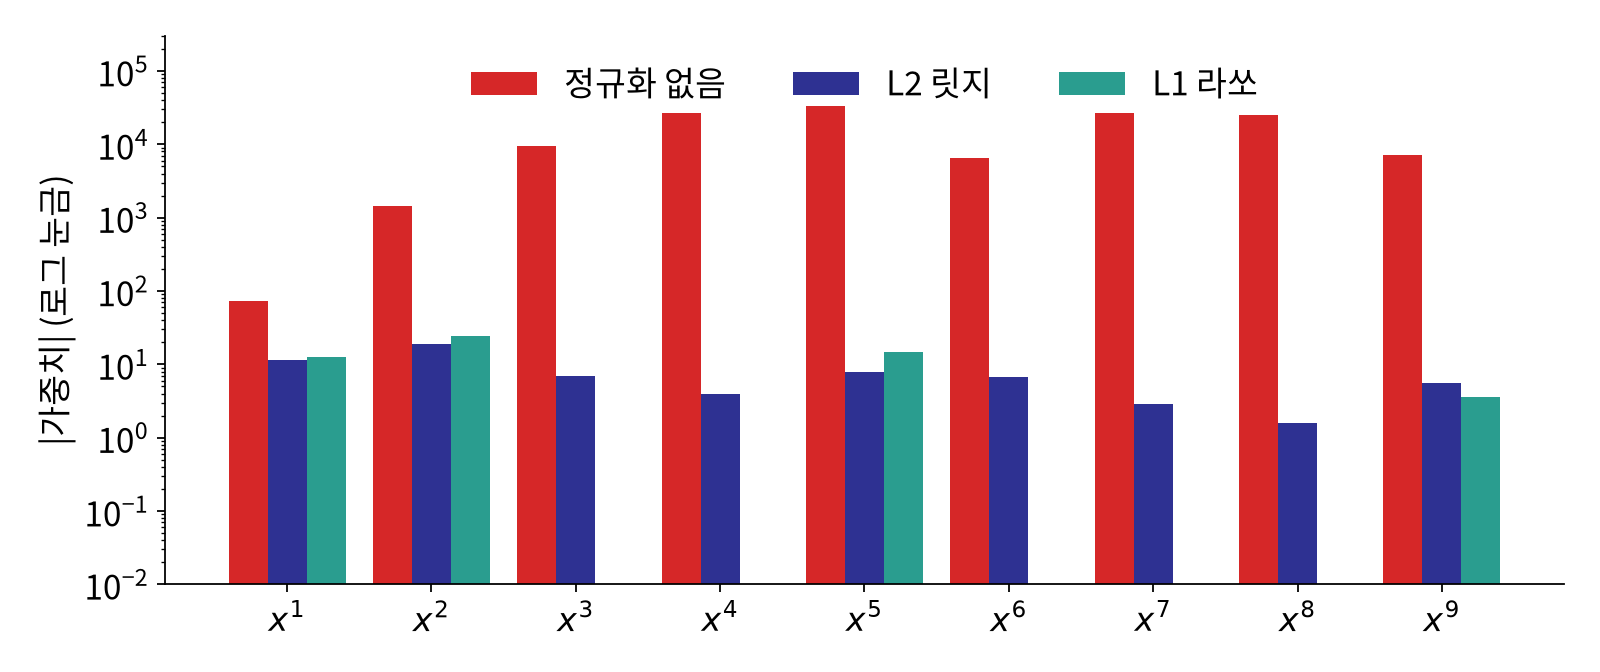
\includegraphics[width=0.8\linewidth]{rg_weights.png}\par\vskip0.2em
{\large 가장 큰 가중치: \; 정규화 없음 \kq{33,589} \quad L2 릿지 \kb{19} \quad L1 라쏘 24 \qquad ($\lambda = 0.005$)}
\vfill
\note{기온 데이터로 돌아가 람다 0.005로 정규화했습니다. 세로축이 로그 눈금이라는 점에 주의하세요. 정규화가 없으면 가중치들이 수백에서 3만 3천까지 갑니다. 릿지를 쓰면 가장 큰 가중치가 19, 라쏘는 24로 천 배 이상 작아집니다. 라쏘의 막대 몇 개는 아예 바닥에 붙어 있는데, 0이라서 그렇습니다. 잠시 뒤에 봅니다.}
\end{frame}

% --- 릿지 곡선
\begin{frame}{L2 릿지: 곡선이 부드러워진다}
\vfill
\centering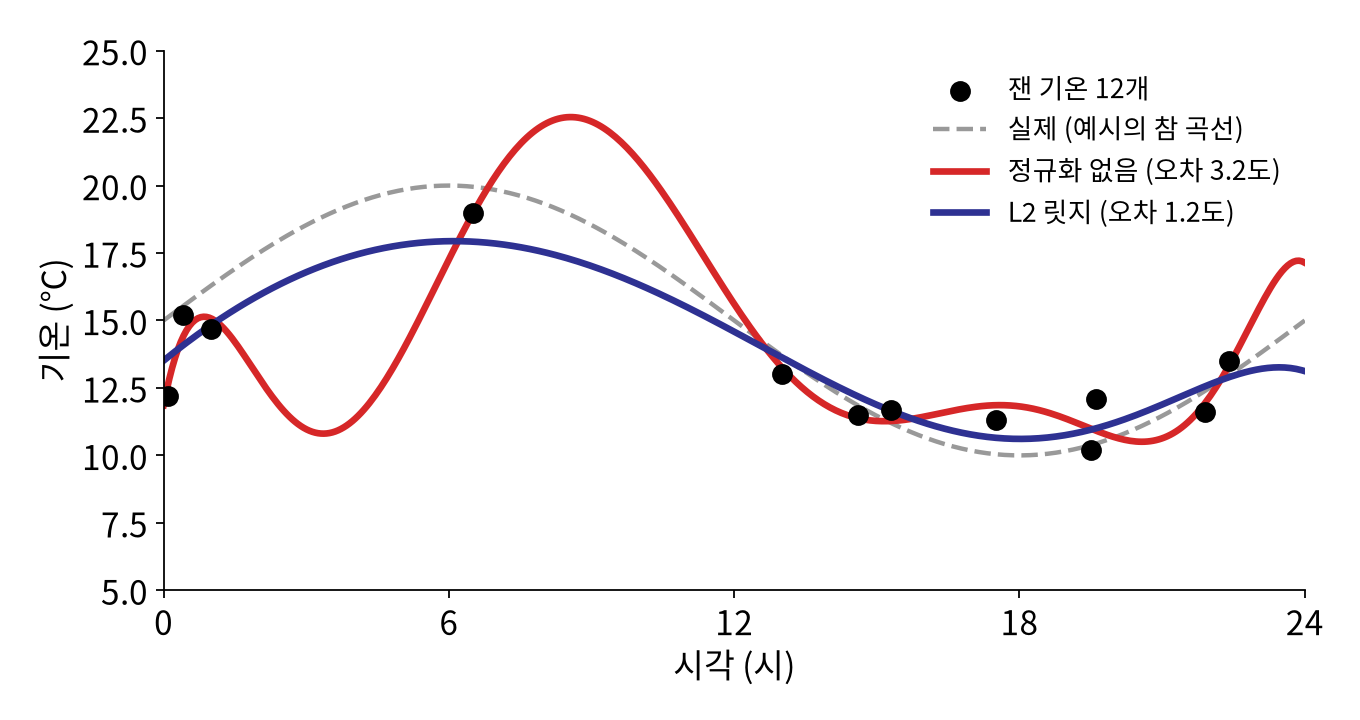
\includegraphics[width=0.62\linewidth]{rg_ridge.png}\par\vskip0.2em
{\large 실제 기온과 오차 \kq{3.2 도} $\to$ \kb{1.2 도} \qquad 잰 점과 오차는 0.57 $\to$ 0.86 도}
\vfill
\note{릿지로 맞춘 파란 곡선입니다. 출렁임이 사라지고 실제 기온 곡선을 꽤 잘 따라갑니다. 실제 기온과 오차는 3.2도에서 1.2도로 줄었습니다. 대신 잰 점 12개와의 오차는 0.57에서 0.86도로 조금 늘었습니다. 점을 덜 외우고 규칙을 배운 겁니다. 차수는 그대로 9차인데도 과대적합이 크게 줄었습니다.}
\end{frame}

% --- 라쏘
\begin{frame}{L1 라쏘: 가중치가 아예 0 이 된다}
\markpage{lasso}
\vfill
\centering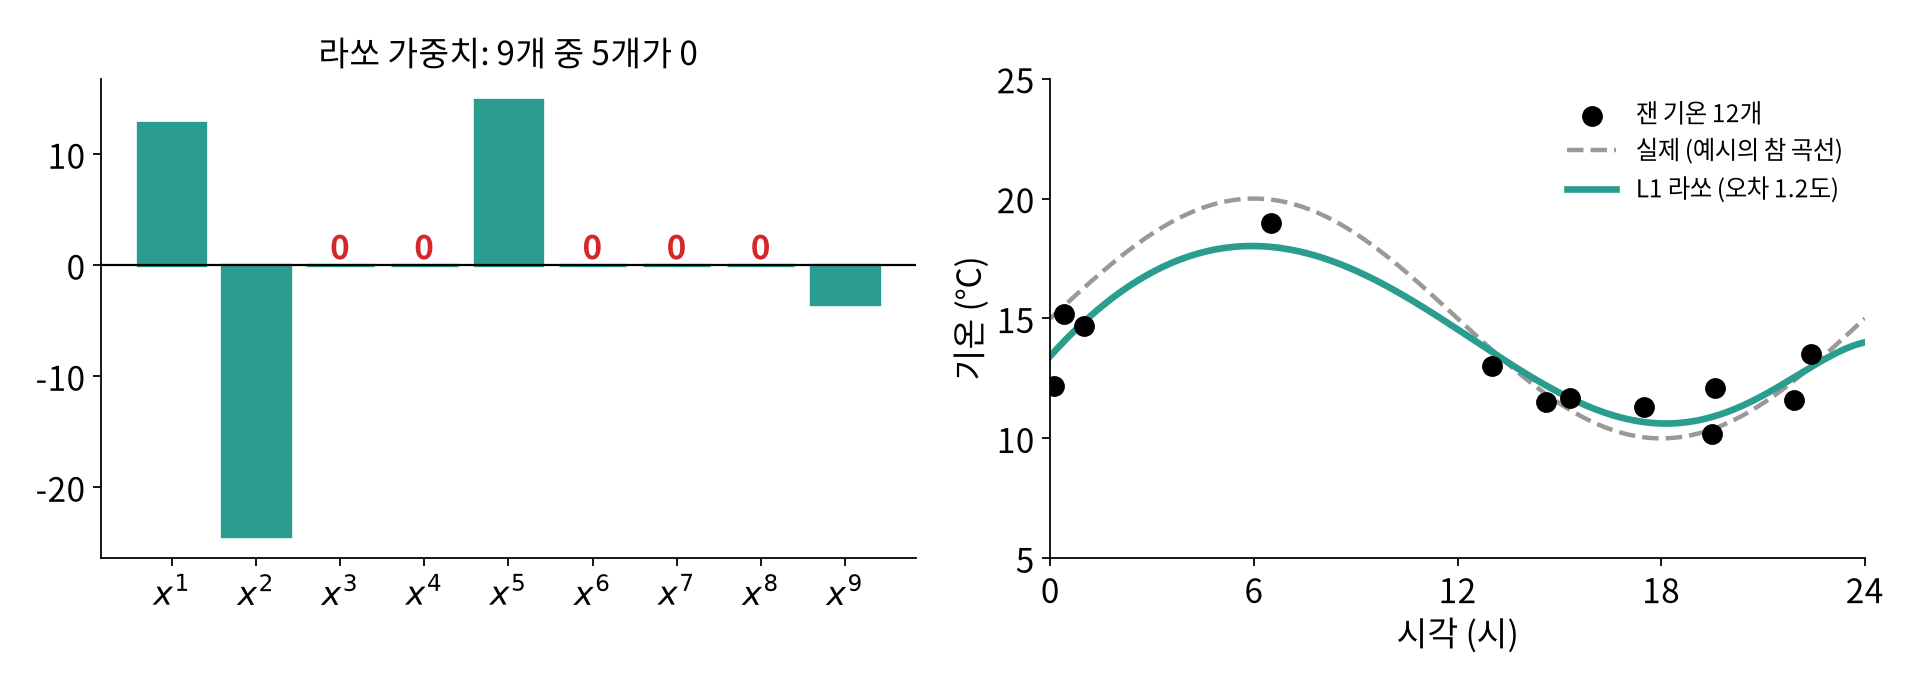
\includegraphics[width=0.86\linewidth]{rg_lasso.png}\par\vskip0.2em
{\large 9개 중 \kq{5개가 정확히 0} \quad 남은 4개로도 오차 \kb{1.2 도} \quad $\to$ 특징 고르기}
\vfill
\note{라쏘는 다른 일을 합니다. 가중치 9개 중 5개를 정확히 0으로 만듭니다. 그 특징을 아예 쓰지 않는다는 뜻입니다. 남은 4개만으로도 실제 기온과 오차는 1.2도로 릿지와 비슷합니다. 라쏘는 정규화를 하면서 동시에 특징을 골라 줍니다. 특징이 수백 개인데 그중 몇 개만 중요할 것 같을 때 특히 유용합니다. 어떤 특징이 살아남았는지가 해석에도 도움이 됩니다.}
\end{frame}

% --- 기하
\begin{frame}{왜 L1 만 정확히 0 이 되나: 원과 마름모}
\markpage{geo}
\vfill
\centering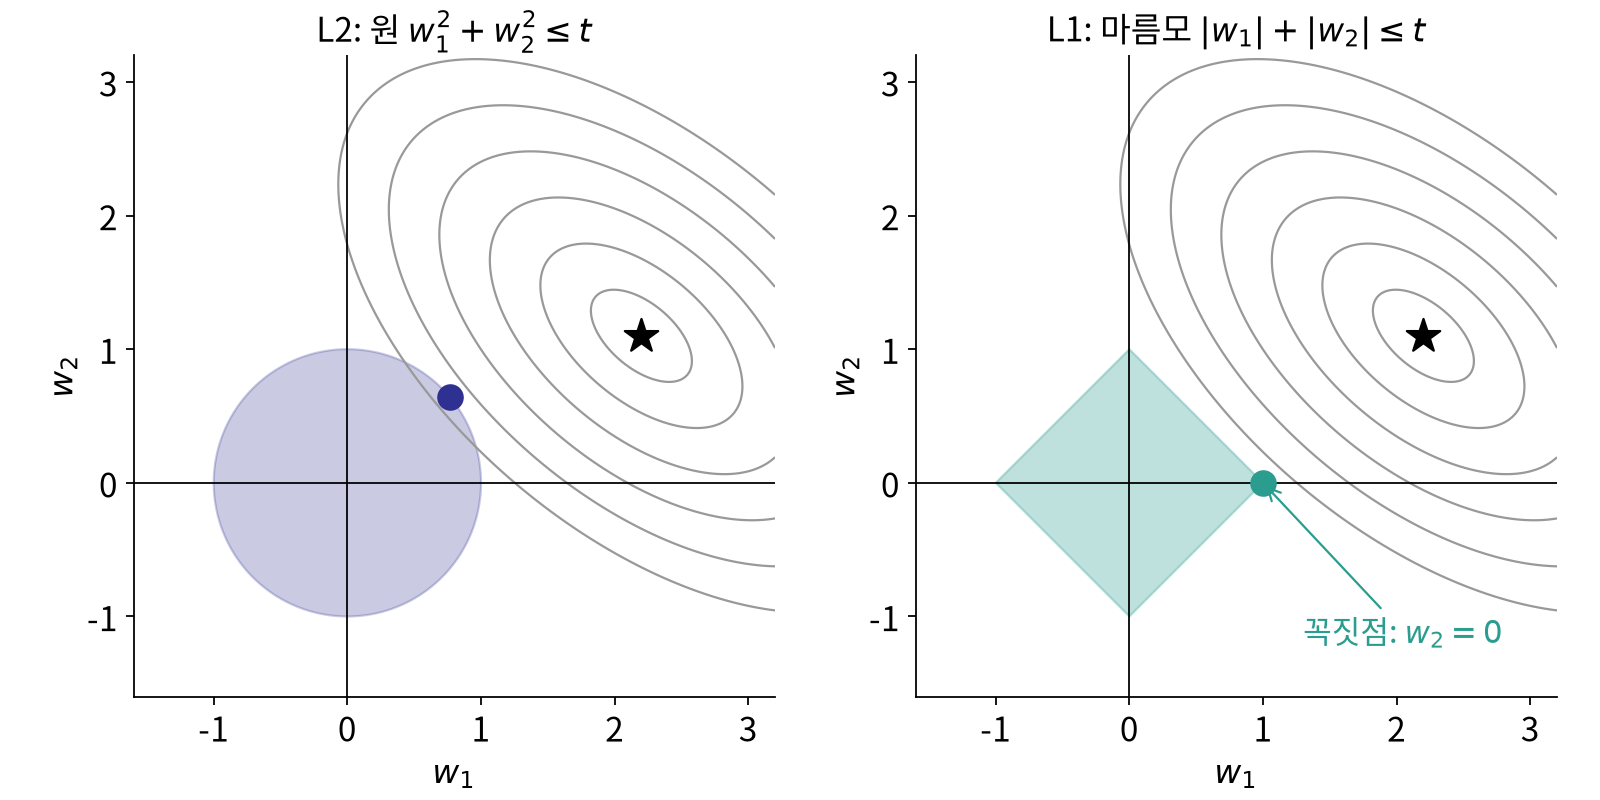
\includegraphics[width=0.66\linewidth]{rg_geo.png}\par\vskip0.2em
{\large 등고선 (타원) 이 영역에 처음 닿는 곳이 답 \quad 마름모는 \kb{꼭짓점}이 축 위}
\vfill
\note{왜 L1만 정확히 0이 될까요? 가중치가 둘인 경우를 그려 봅니다. 회색 타원은 오차의 등고선이고, 별이 정규화 없는 답입니다. 정규화는 가중치가 색칠한 영역 안에 있어야 한다는 조건과 같습니다. L2는 원, L1은 마름모입니다. 답은 타원을 점점 키울 때 영역에 처음 닿는 곳입니다. 원은 둥글어서 보통 축이 아닌 곳에서 닿습니다. 그래서 두 가중치가 모두 작아질 뿐 0이 되지는 않습니다. 마름모는 뾰족한 꼭짓점이 축 위에 있어서, 타원이 꼭짓점에 먼저 닿기 쉽습니다. 꼭짓점에서는 w2가 정확히 0입니다.}
\end{frame}

% --- 경로
\begin{frame}{$\lambda$ 를 키워 가면: 계수 경로}
\vfill
\centering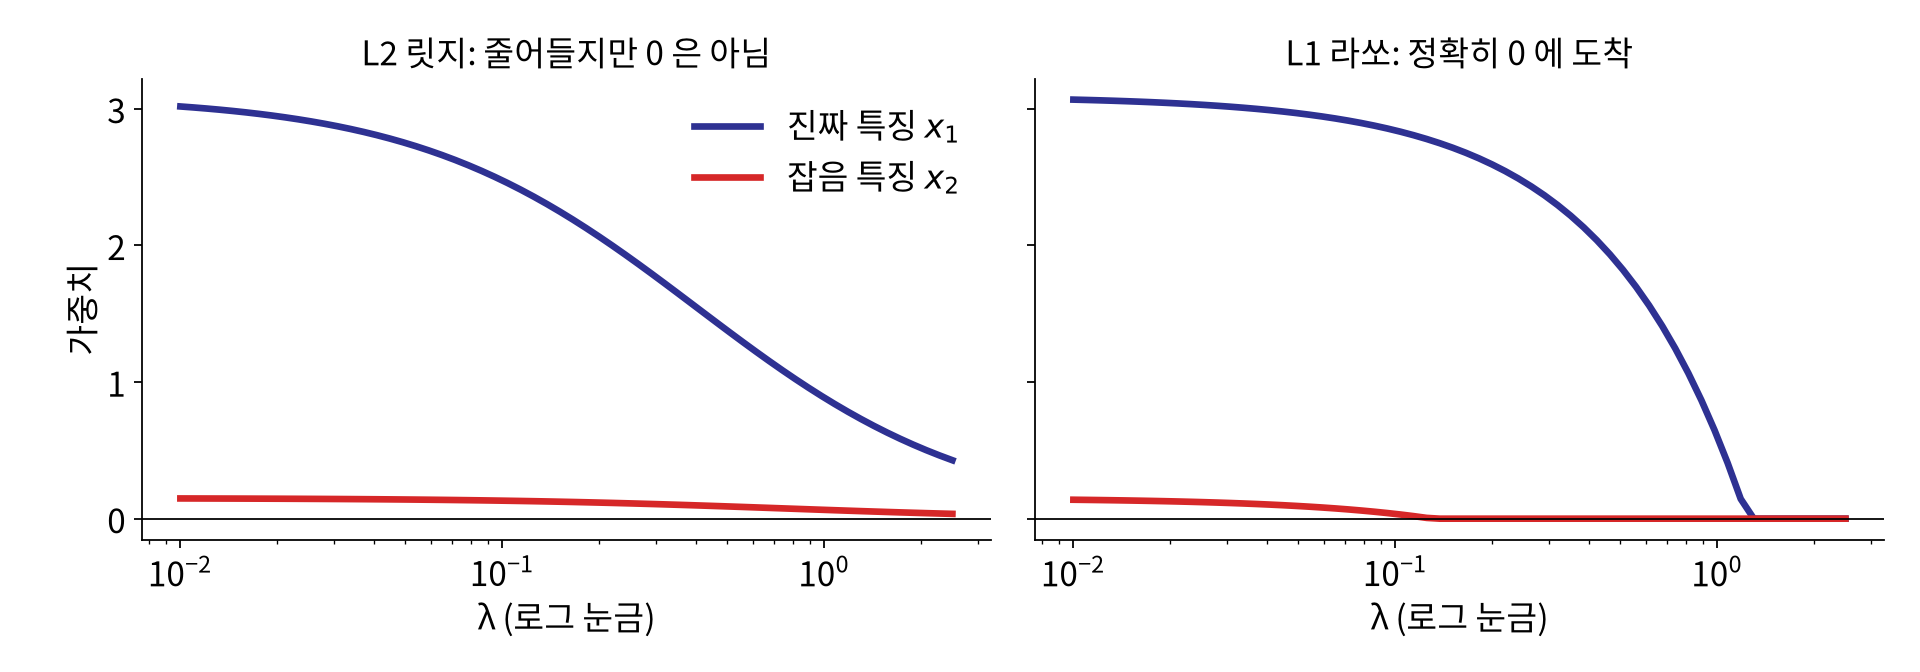
\includegraphics[width=0.84\linewidth]{rg_path.png}\par\vskip0.2em
{\large 잡음 특징 $x_2$: 릿지는 \textbf{계속 작아질 뿐}, 라쏘는 \kq{$\lambda \approx 0.13$ 에서 0 에 도착}}\\[0.2em]
{\small 진짜 특징 $x_1$ ($y = 3x_1 + $ 잡음) 은 끝까지 살아남다가, 벌금이 아주 세지면 그제야 0 \quad (점 30개 예시)}
\vfill
\note{특징이 두 개뿐인 예로 람다를 0.01부터 2.5까지 키워 봤습니다. x1은 y를 실제로 만드는 진짜 특징이고, x2는 아무 관련 없는 잡음 특징입니다. 릿지는 람다를 키우면 두 가중치가 모두 서서히 작아지지만 0이 되지는 않습니다. 라쏘는 잡음 특징 x2가 람다 0.13 근처에서 정확히 0에 도착하고 그 뒤로 계속 0입니다. 진짜 특징 x1은 끝까지 버티다가 벌금이 아주 세지면 그제야 0이 됩니다. 라쏘에서 0은 서서히 다가가는 값이 아니라 도착하는 곳입니다.}
\end{frame}

% --- lambda 손잡이
\begin{frame}{$\lambda$ 는 손잡이: 너무 약하면 출렁, 너무 세면 납작}
\markpage{sweep}
\vfill
\centering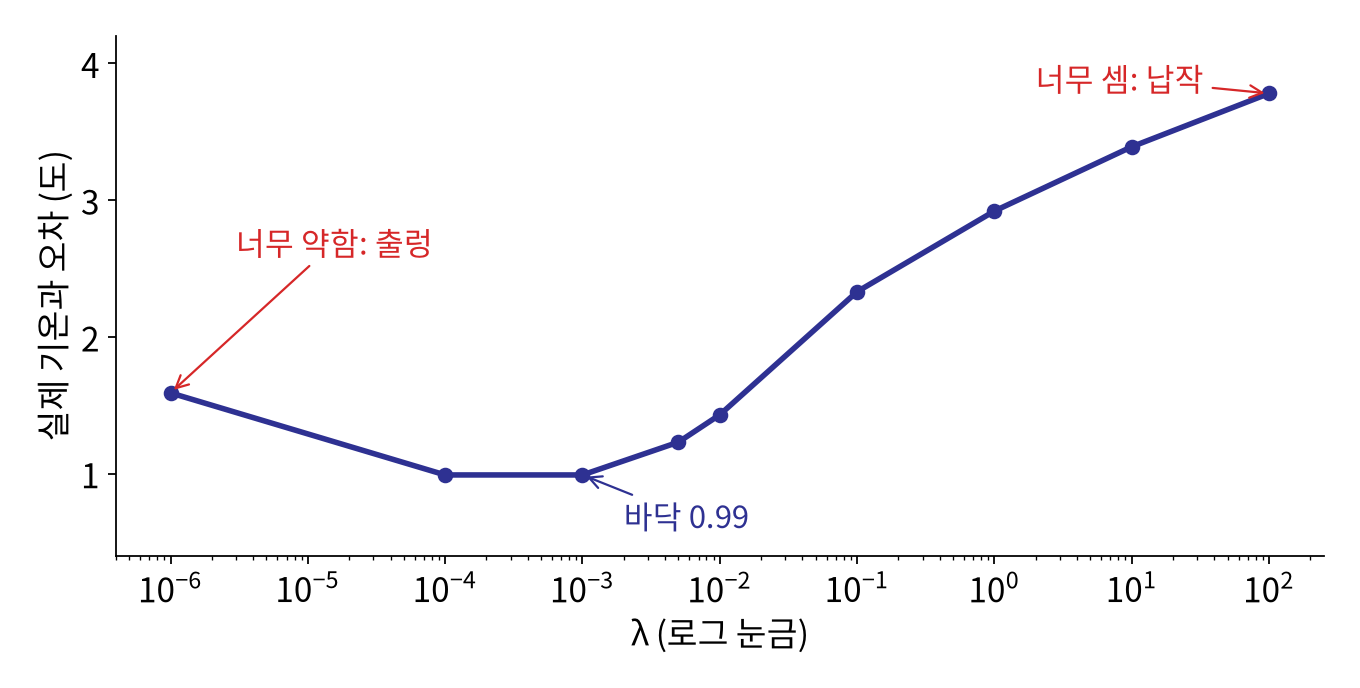
\includegraphics[width=0.6\linewidth]{rg_sweep.png}\par\vskip0.2em
{\large $\lambda$: $10^{-6}$ \kq{1.59 도} $\to$ $10^{-3}$ \kb{0.99 도} $\to$ $100$ \kq{3.78 도} \qquad U 자의 바닥을 찾아야 한다}
\vfill
\note{람다를 바꿔 가며 실제 기온과의 오차를 그렸습니다. 람다가 너무 작으면 벌금이 거의 없어서 곡선이 출렁이고 오차가 1.59도입니다. 과대적합입니다. 람다가 너무 크면 가중치를 다 눌러서 곡선이 평평해지고 오차가 3.78도입니다. 과소적합입니다. 그 사이 람다 0.001 근처에서 0.99도로 가장 작습니다. U자 모양이고 우리는 그 바닥을 찾아야 합니다. 그런데 실제 문제에서는 회색 점선 같은 정답 곡선이 없습니다. 바닥을 어떻게 찾을까요? 다음 시간의 교차 검증이 답입니다.}
\end{frame}

% --- 문제풀이
\begin{frame}{문제풀이}
\vfill
\begin{enumerate}
\item 가중치 $\mathbf{w} = (3, -4)$ 의 L2 벌금 $\sum w_j^2$ 과 L1 벌금 $\sum |w_j|$ 은? $\lambda = 0.1$ 이면 손실에 더해지는 값은 각각?\vskip0.8em
\item 손 계산 예 \pref{hand} 에서 $\lambda$ 를 아주 크게 하면 $(w_0, w_1)$ 은 어디로 가나?\vskip0.8em
\item 특징 200개 중 실제로 중요한 것이 5개쯤이라고 생각된다. L1 과 L2 중 무엇을 먼저 써 보겠나?\vskip0.8em
\item 정규화한 모델의 학습 오차가 정규화하지 않은 모델보다 크다. 잘못된 것인가?
\end{enumerate}
\vfill
\note{1번 답. L2는 9 더하기 16, 25이고 L1은 3 더하기 4, 7입니다. 람다 0.1이면 각각 2.5와 0.7이 더해집니다. 2번 답. 기울기는 0으로, 절편은 y의 평균 5로 갑니다. 평평한 직선 y는 5입니다. 3번 답. L1, 라쏘입니다. 쓸모없는 195개의 가중치를 0으로 만들어 줄 가능성이 큽니다. 4번 답. 아닙니다. 정규화는 학습 오차를 조금 희생해서 새 데이터 오차를 줄이는 방법이라, 학습 오차가 커지는 게 정상입니다.}
\end{frame}

% --- 실습
\begin{frame}{실습}
\vfill
\centering\begin{tabular}{rl}
\large 1 & 릿지 정답 식 직접 구현 $\to$ 손 계산 $(3, 1)$, $(4.33, 0.33)$ 재현 + 기온 9차 곡선\\[0.5em]
\large 2 & 잡음 특징 실험: 릿지는 작아지고, 라쏘는 정확히 0\\[0.5em]
\large 3 & 실제 데이터: 당뇨병 환자 442명, 특징 10개 중 라쏘가 고르는 것
\end{tabular}\vskip1em
Diabetes (Efron et al., 2004; scikit-learn) \\[0.4em]\href{https://colab.research.google.com/github/SuminHan/book-ml/blob/main/slides/v2/ml1/week06/regularization/lab/regularization.ipynb}{\textcolor{ksagolddk}{▶ Colab에서 실습 노트북 열기}}
\vfill
\note{실습은 세 부분입니다. 첫째, 릿지의 정답 식을 numpy로 직접 구현해서 손 계산 결과를 재현하고, 기온 데이터의 9차 곡선을 길들여 봅니다. 둘째, 진짜 특징과 잡음 특징이 섞인 데이터로 릿지와 라쏘의 계수 경로를 직접 그립니다. 셋째, 당뇨병 환자 442명의 나이, BMI, 혈압, 혈액 검사 수치 10개로 1년 뒤 병의 진행 정도를 예측하면서, 라쏘가 람다에 따라 어떤 특징을 먼저 남기는지 봅니다.}
\end{frame}

% --- 정리
\begin{frame}{정리}
\vfill
\centering\large\begin{tabular}{l}
과대적합의 증상: 가중치가 엄청나게 크다\\[0.5em]
\textbf{정규화} \quad 손실 + $\lambda \times$ 가중치 벌금 \quad (절편은 제외)\\[0.5em]
\kb{L2 릿지} $\sum w^2$: 모두 작게 \qquad \kb{L1 라쏘} $\sum |w|$: 일부를 정확히 0 (특징 고르기)\\[0.5em]
$\lambda$ 는 손잡이: 약하면 과대적합, 세면 과소적합 $\to$ \textbf{교차 검증}으로 고른다
\end{tabular}
\vfill
\note{정리합니다. 과대적합된 모델은 가중치가 엄청나게 크다는 증상이 있습니다. 정규화는 손실에 람다 곱하기 가중치 벌금을 더해서 가중치를 작게 유지시킵니다. 절편은 빼고요. 제곱 벌금인 릿지는 모든 가중치를 고르게 줄이고, 절댓값 벌금인 라쏘는 일부를 정확히 0으로 만들어 특징을 골라 줍니다. 람다는 손잡이라서 약하면 과대적합, 세면 과소적합이 되고, 그 바닥은 다음 시간에 교차 검증으로 찾습니다.}
\end{frame}
\end{document}
